\clearpage\PageTitle{Contact localization and clamp reactions}
\begin{center}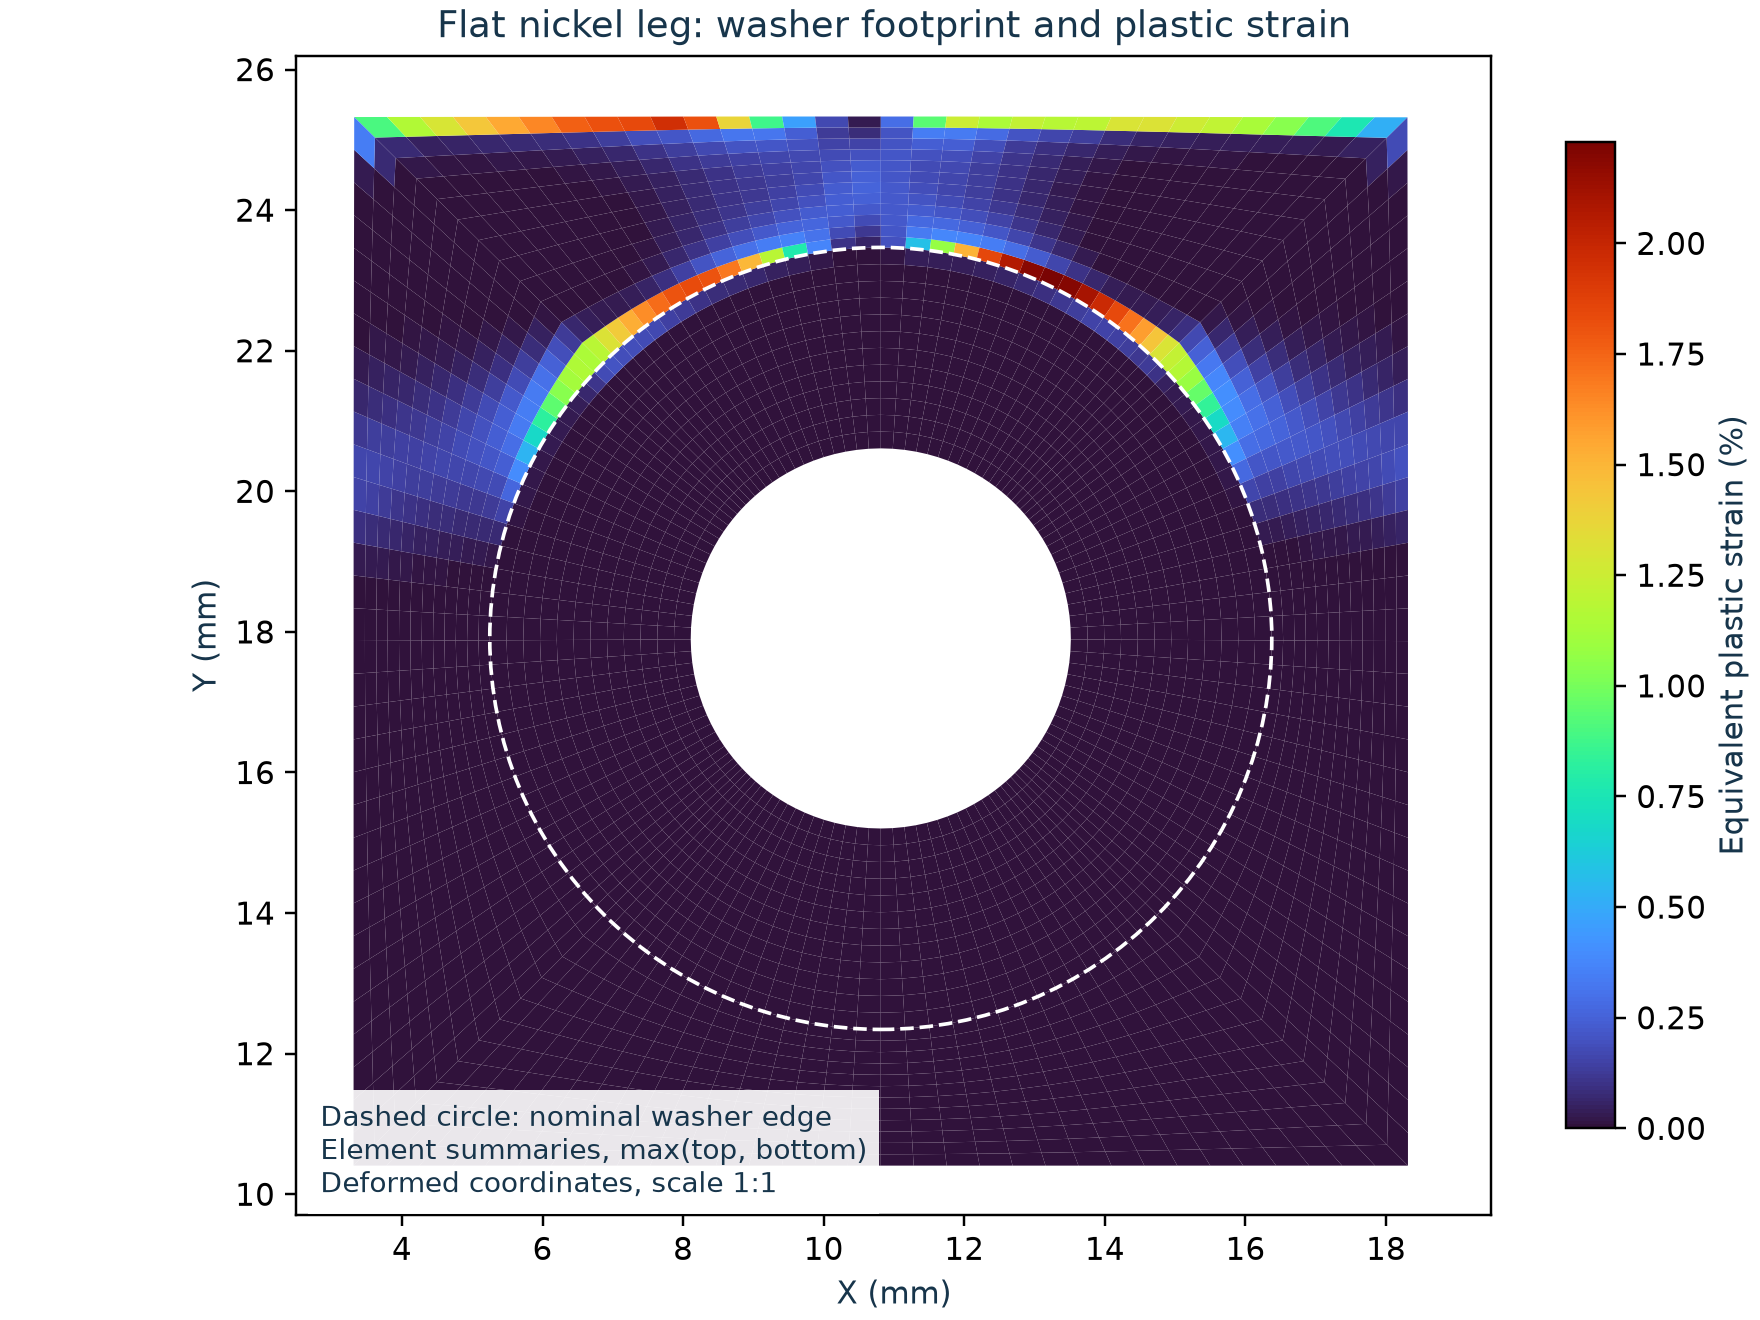
\includegraphics[width=.76\linewidth,height=102mm,keepaspectratio]{figures/friction_locked_fine_plastic_plan.png}
\captionof{figure}{Refined 750 N contact model at $u_X=+0.5$ mm. The lower nickel flat leg is shown in deformed coordinates at scale 1:1. Colour is the maximum of top/bottom shell element-summary plastic strain, not a fracture index.}\end{center}
\begin{center}\begin{tikzpicture}\begin{axis}[width=.98\linewidth,height=56mm,xlabel={Battery centre displacement (mm)},ylabel={Normal platen reaction (N)},xmin=0,xmax=.5,grid=both,legend style={font=\footnotesize,at={(.03,.97)},anchor=north west},xticklabel style={/pgf/number format/fixed,/pgf/number format/precision=2},tick label style={font=\small},label style={font=\small}]
\addplot+[color=Teal,thick,mark=none] table[col sep=comma,x=u,y=washer1] {data/friction_locked_clamp.csv};\addlegendentry{Coarse mesh}
\addplot+[color=Navy,thick,mark=none] table[col sep=comma,x=u,y=washer1] {data/friction_locked_fine_clamp.csv};\addlegendentry{Fine mesh}
\end{axis}\end{tikzpicture}

\captionof{figure}{Normal reaction at the first lower platen during the pull; the second platen gives essentially the same result. Both start at 750 N after the force-to-lock transfer. The fixed platen separation permits reaction to change under bending.}\end{center}
The refined contact calculation reports a maximum element-averaged penetration of 0.424 micrometres (0.283\% of strip thickness) over its saved history. The greatest accumulated plastic slip among the exported contact corner values is 1.071 micrometres. These contact quantities use a different sampling convention from the element-averaged sliding in the main table.\par
The pressure and sliding depend on the assumed friction coefficient, contact stiffness and rigid support idealization. Their numerical convergence and constitutive calibration are distinct questions. Small penetration is a numerical contact check; it does not establish that the real nickel, washer or PCB avoids indentation or tearing.
